\documentclass[language=chinese]{hustproposal}

\department{计算机科学与技术学院}
\title{基于Android平台的网络防火墙的设计与实现}
\author{易亚洲}
\major{信息安全}
\supervisor{李平}{讲师}

\begin{document}

\section{课题目的和意义}

随着智能手机的普及,以及4G网络的快速发展,越来越多的用户开始使用手机上网冲浪。中国互联网络信息中心(CNNIC)发布了第38次《中国互联网络发展状况统计报告》。《报告》显示,截至2016年6月,中国网民规模达7.10亿,其中手机网民规模达6.56亿,占比达92.5\%。中国各类第三方市场鱼龙混杂,管理混乱,对应用上架的审核存在不规范,不严格甚至完全没有审核的现象。

根据赛门铁克(Symantec)最新互联网安全威胁报告称,在所有的安卓应用程序中有17\%是恶意软件。特别是Google Play市场无法提供服务的地区,用户不得不从未知来源下载安全应用,各种第三方市场鱼龙混杂,其中有很多恶意软件混迹其中,也有很多安全性低容易收到攻击的应用。

\begin{figure}[h!]
\centering
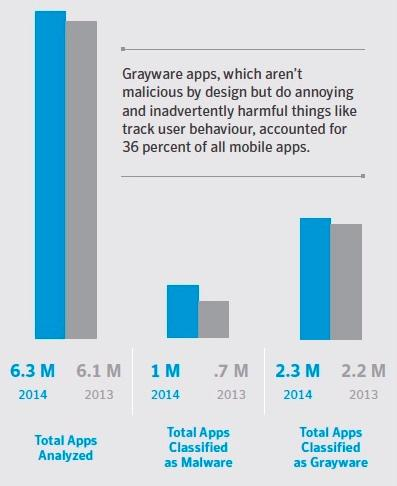
\includegraphics[width=.4\textwidth]{images/symantec_report}
\caption{Symantec恶意软件数量报告}\label{fig:2}
\end{figure}

腾讯移动安全实验室发布了2016年手机安全报告,报告显示2016年Android病毒包共增加2341.8万,同比增长40.20\%。2016年Android手机病毒感染用户数同比增长62.43\%,感染用户数总量达到5亿人次,达到历年新高。其中资费消耗类占比高达84.24\%,在2016年手机病毒类型中排名第一。
资费消耗类的病毒是指的在未经用户授权的情况下,通过频繁连接网络、发送短信等方式,导致用户资费损失。这部分病毒往往帮助一些广告商提高App装机量或点击率进行恶意推广,不断联网下载,消耗用户流量。

针对资源消耗类病毒,网络防火墙可以启动有效的防范和遏制的作用,将不可信应用的网络权限进行限制,对可疑应用的数据通信进行监控,是遏制这类病毒的最重要手段。此外,对于远程控制、隐私窃取等类型的软件,限制网络通信也是有效可行的重要举措。

Android系统自带的通信权限管理仅仅允许对特定应用设置是否允许链接网络,无法对Wifi网络和蜂窝数据网络区分设置,也不支持多种条件下的自定义规则,如灭屏和亮屏,特定网络,限制时段等条件,而且,不支持按协议过滤,按源目的地址过滤等基本防火墙功能。所以我们有必要开发一款Android网络防火墙来完善这些功能,满足用户对Android网络管理更高级的需求。
所以在目前Android用户数量持续增长,资费消耗病毒日渐猖獗,而Android系统网络功能不全的情况下,所以我们提出了设计并实现一个基于Android平台的网络防火墙的课题,旨在通过对Android系统网络通信的监控和管理的实现,研究Android网络安全,设计一个可用的Android网络防火墙,改善Android系统的安全性。


\section{国内外研究现状和发展趋势}

实现对Android流量的过滤,有多种实现方式.

Android内核是linux内核的一种分支,也提供netfilter和iptable,可以参考Linux内核防火墙的实现方式实现Android防火墙。Netfilter是Linux 2.4.x之后版本提供的包过滤的框架,它在TCP/IP协议栈中提供了相应的Hook,允许我们对网络数据包进行过滤,丢弃,修改等操作。通过netfilter中的一些函数即可实现防火墙应用。而iptables是linux提供的一个基于netfilter工具,使用户可以对整个操作系统收发的数据包就行拦截修改拒绝等操作。

另外,Android系统本身提供了制作VPN应用的API,允许第三方应用向系统提供VPN,系统负责将网络流量转发到VPN应用,VPN应用可以建立隧道实现VPN服务。而在这个过程中,VPN应用可以对网络流量进行分析和过滤,实现防火墙的功能。
netfilter/iptable需要调用netfilter api或执行iptable,这都必须拥有root权限才有可能实现。Root本身就是利用漏洞才得以实现的,并且root之后的手机毫无安全性可言,与我们做防火墙提高安全性的初衷相悖。VPN方案由于使用了Android官方提供的公开API,可以不需要Root权限运行,只需要用户在第一次启动VPN时授予许可,也没有给系统带来额外的安全风险。其缺陷在于VPN服务只允许启动一个,将会导致用户使用防火墙后无法使用其他VPN。

以加强Android安全作为出发点,通过对两种方案的对比,我们最后决定采用VPN方案实现Android防火墙。

除了根据配置对网络行为管理的传统防火墙,最近的研究更多将注意力放在里将传统防火墙和其他安全技术相结合的方案。

在最新的研究中,研究者往往采用多种其他技术实现对应用程序的可信度进行评估,防火墙成为利用评估结果,实现对不可信应用程序或异常行为的组织和控制的手段。如
Najim Ammari* , Almokhtar Ait El Mrabti, Anas Abou El Kalam, Abdellah Ait Ouahman等人提出了一种解决敏感数据泄漏的防火墙,他们提出的方案利用数据挖掘对大量应用程序二进制文件进行静态分析,通过对敏感操作的钩子代理来对应用程序的危险程度进行动态分析,最后分析结果作为一个关键参数,用于决策防火墙的行为。与传统防火墙不同的是,他们提出的防火墙引入的信任机制。最后结合可信数据和分析数据进行决策。


而还有一部分研究,不仅将防火墙作为最终控制和组织威胁的手段,而开始将防火墙作为一种识别威胁的信息源。

Tendai Munyaradzi Marengereke和K. Sornalakshmi的提出的一个基于云的Android安全监控的收集系统,实现对异常网络流量的监控,响应和处理,其根本就是在于实现网络防火墙流量监控和网络管理,防火墙即是对威胁进行处理和阻止的主体,也是在发现威胁前,进行信息收集的主体。




\section{预期目标}


本论文的目标是通过设计和实现一个Android网络防火墙,通过对Android系统网络通信的监控和管理,提高Android系统的安全性,有效防范资费消耗类恶意软件。目前存在多种Android防火墙的实现方案,但我们希望避提供一个普通Android用户下载安装后即可用的解决方案,而不是要求提取系统Root权限,甚至定制操作系统内核等难以实行的方案。本文采取的设计方案不是类似传统防火墙由管理员设定一组规则然后一直照此执行直到修改规则,而是采用交互式规则,在应用尝试进行一些网络请求时,通知用户做出决策:允许或者拒绝,并且即时的更新规则。同时需要监控连接的流量消耗,提供地址的相关信息,为用户做出决策提供帮助。


最后,将针对防火墙的性能,对处理每个包时引入的能耗,包丢失和延迟进行基准测试。通过分析证明,使用这样的防火墙是可行的,并且不影响Android设备的日常功能。

\section{研究内容及核心技术}


在对市场上多款防火墙类应用软件进行分析和比较之后,将用户需求列为以下几点:
\begin{itemize}
	\item 过滤Android系统所有流量\label{item:1}
	\item 图形界面,操作简便,通俗易懂
	\item 支持WiFi和数据流量应用不同规则
	\item 支持亮灭屏状态应用不同规则
	\item 支持分时段应用不同规则p
\end{itemize}

对于上述需求,进行明确和细化,方便开发和测试验收:
\subsection{功能性要求}
\subsubsection{兼容和适配}

	兼容到Android4.0及以上
\subsubsection{防火墙}
\begin{enumerate}
	\item 交互式规则:如果新建立的连接没有已知的规则进行决策,会通知用户即时作出决策。在用户可以在弹出的通知栏里选择允许或者拒绝,然后就会记住该规则,在以后有相同的连接时采用该规则;如果用户选择了拒绝,该连接将会被切断。
	\item 审计式规则:用户可以查看近期所有的连接记录,可以选择对特定连接快捷建立规则
	\item 规则的适用范围:
		\begin{itemize}
			\item 面向应用:用户可以设定规则只对特定应用生效
			\item 面向出口:用户可以设定规则只对特定网络环境生效,如Wifi/2G/3G/LTE/漫游
			\item 面向特定状态:用户可以设定规则只对特定手机状态生效
		\end{itemize}
	\item 防火墙默认策略:当用户没有为特定应用设定规则时,采用默认策略
	\item 实时网速监控:用户可以在通知栏查看实时的网速
	\item 新应用提示:在用户安装新的应用程序后,会提示用户为其创建规则
\end{enumerate}

\subsubsection{性能}

网络防火墙为了提供额外的安全保障,必须尽可能的持续运行。所以网络防火墙必须对Android移动设备的的性能和电量的消耗保持在最小。所以必须采取措施将防火墙规则匹配的耗时和对包处理的耗时降到最低,例如TCP连接可以只对SYN和FIN包进行处理便可实现监控TCP连接的生命周期,此外我们还需对其他协议及在所有可能的环节降低性能损失,并通过性能测试和报告证明防火墙对设备所造成的性能损失在可以容忍的较小范围之内。

\subsection{非功能性要求}

为了提高体验和方便实际使用,还需实现一些非核心功能的特性:
\begin{enumerate}
	\item 日志查看:记录应用程序的网络访问尝试
	\item 支持系统应用:支持对系统应用设置规则
	\item 支持IPv6:提供对IPv6及ICMPv6的支持
	\item 端口转发:支持增加/删除/编辑端口转发规则
	\item 配置导入导出:支持将规则和配置导出到文件或者从文件中导入
	\item 持久有效:防火墙必须持续有效的工作:\begin{itemize}
		\item 进程必须尽可能避免被系统停止或杀死
		\item 防火墙必须在断开时尝试重新启动
		\item 防火墙必须在开机自动启动
	\end{itemize}
\end{enumerate}



\section{课题研究进度安排}


项目的工作主要安排在2017年2月13日至2017年5月22日。相关重要时间点如下:
\begin{enumerate}
	\item 开题,第四周前(2017年3月10日前)
	\item 中期检查,第九周前(2017年4月10日前)
	\item 完成论文编写,第15周前(2017年5月22日前)
	\item 答辩和验收,第18周前(2017年6月16日前)
\end{enumerate}

具体时间及任务安排如下:

\begin{table}[h!]
\centering
\caption{研究进度安排表}
	\begin{tabular}{|c|l|l|}\hline
	周次 	& 日期 & 任务安排\\\hline
	1		& 2.13~2.19 & 收集相关文献,对Android安全和防火墙技术的最新研究进行了解,编写文献综述\\\hline
	2		& 2.20~2.26 & 体验和研究现有的防火墙应用,进行市场调查\\\hline
	3		& 2.27~3.5  & 完成需求分析,确定方案可行性,了解项目要求的技术知识\\\hline
	4		& 3.6 ~3.10 & 完成开题报告\\\hline
	5		& 3.11~3.19 & 完成好相关准备工作,进行总体模块划分,确定各模块的总体设计\\\hline
	6,7		& 3.20~4.2  & 编码实现,完成核心功能\\\hline
	8,9 	& 4.3 ~4.16 & 编码实现图形界面\\\hline
	10		& 4.17~4.23 & 进行基本功能的测试\\\hline
	11,12	& 4.24~5.7  & 增加更多功能,完善兼容性,性能优化和改善易用性\\\hline
	13 		& 5.8 ~5.14 & 进行完整的功能测试,兼容性测试和性能测试\\\hline
	14 		& 5.15~5.22 & 对开发工作进行整理,编写论文报告\\\hline
	\end{tabular}
\end{table}

\nocite{*}
\bibliography{proposal_ref}

\end{document}
\endinput
